\chapter{wafamole++}
\label{chp:capitulo4}

Tendo em consideração o embasamento teórico estabelecido e a oportunidade de contribuir para um projeto \textit{open source} na área de interesse deste trabalho que tivesse uma boa abrangência e impacto, foi concebido o \textbf{wafamole++}, uma versão estendida do WAF-A-MoLE anteriormente descrito no capítulo de Revisão de Literatura. Foram seguidas diretrizes e recomendações de contribuição estabelecidas pelos autores, e alguns módulos adicionais contendo funcionalidades não disponibilizadas pelos mesmos referentes ao treinamento de novos classificadores, geração de novos modelos, e tratamento de datasets foram disponibilizados com este trabalho.

A elaboração do mesmo permitiu um entendimento mais profundo da ferramenta original, recebendo apoio dos autores originais e atualmente conta com uma série de operadores de mutação novos e sobretudo modelos de classificadores novos implementados para um Web Application Firewall de código aberto encontrado na plataforma de colaboração Github.

Acredita-se que essa colaboração ocasionou em uma ferramenta mais abrangente, com uma menor barreira de entrada para futuros colaboradores e mais flexível para avaliação de Web Application Firewalls baseados em Aprendizado de Máquina no geral. Assim espera-se que mais contribuições possam ser geridas no futuro, estabelecendo-se como um projeto complementar ao WAF-A-MoLE original.


\section{Arquitetura}

O cerne do projeto encontra-se nos seguintes módulos:
\begin{alineas}
\item \verb+Main+ - Responsável pela lógica da linha de comando, com todos os decorators da biblioteca \verb+Click+ que facilitam o desenvolvimento de utilidades de terminal. É feito o recebimento e passagem de parâmetros para a pipeline do programa aqui, além de ser instanciada a classe principal \verb+wafamole+ e o módulo \verb+EvasionEngine+ com o modelo selecionado pelo usuário.
\item \verb+models+ - Em models estão localizados os modelos de exemplo para experimentação de desenvolvedores novos, modelos padrões do WAF-A-MoLE e sobretudo modelos novos (também customizáveis) introduzidos no wafamole++, localizados na pasta \verb+/models/svc+. Modelos novos de classificadores de Web Application Firewalls a serem testados são tipicamente arquivos .dump das classes de tais classificadores, gerados através biblioteca \verb+joblib+ após o treinamento (no caso do scikit-learn, da função \verb+.fit()+). Alternativamente, essa biblioteca permite também a geração de um arquivo .dump de uma pipeline caso o treinamento exija mais de uma etapa, como uma Tokenização para possibilitar o treinamento de um dado classificador.
\item \verb+EvasionEngine+ - Essa classe contém o loop principal que requisita as mutações responsáveis pela transformação do payload fornecido pelo usuário em um payload considerado inócuo para o WAF avaliado. As requisições são feitas ao módulo \verb+Fuzzer+.
\item \verb+Fuzzer+ - Nesse módulo ficam armazenados os operadores de mutação que transformam o payload a cada rodada de mutação efetuada, e cada mutação ocorre dentro do mesmo. Um operador de mutação aleatório dentre estes é escolhido a cada iteração da pipeline principal.
\end{alineas}

Esses módulos, no entanto, não podem ser trivialmente estendidos sem alguns componentes auxiliares criados para o wafamole++, que são:
\begin{alineas}
\item \verb+datasets+ - Aqui são contidos os datasets SQLiV3, SQLiV4, e SQLiV5, funções de tratamento para os mesmos e uma função de geração/adaptação do dataset original do WAF-A-MoLE para servir de treinamento para o MLBasedWAF, um Web Application Firewall que será descrito na seção seguinte. O SQLiV3 é o primeiro dataset utilizado para tal, disponibilizado pelo Kaggle e também está descrito adiante. Versões subsequentes (indicadas pelos números ascendentes) são incrementos realizados e testados nele com reforços de \textit{payloads} oriundas do wafamole++.

\begin{alineas}
\item \verb+mole+ - A função apelidada de \textit{mole} executa na linha de comando o WAF-A-MoLE para cada linha do dataset SQLiV3, de modo a gerar um leque mais amplo de ataques. Como se trata de um processo iterativo, um limite superior de 7000 novos payloads foi adotado - e o tempo de execução médio foi em torno de 8 horas para o processo todo. Para gerar novos ataques (dado que o WAF-A-MoLE produz saídas diferentes a cada execução), basta executá-lo com redireção de output padrão \textbf{>} \verb+./mole_query_generator.py > output.json+.

\item \verb+sqli_cleaner+ - Essa função auxiliar foi codificada inicialmente com a finalidade de transformar o dataset SQLiV3 do formato .csv para .json que seria mais simples de trabalhar em Python, além de adaptá-lo para o padrão visto no MLBasedWAF, porém uma série de inconsistências suscitou um polimento e tratamento de certos casos para que a saída fosse corrigida. Seu código está disponível nessa seção.

\item \verb+wafamole_dataset_generator+ - Fornecido apenas após um certo período de espera, o dataset do wafamole é disponibilizado no seu \href{https://github.com/zangobot/wafamole_dataset}{repositório} de maneira modular - com uma série de arquivos .json pequenos devido ao limite imposto pela plataforma Github. Além disso, ele precisou ser adaptado para o formato do MLBasedWAF assim como o SQLiV3 (sem grandes dificuldades nesse caso). Possui uma abrangência e riqueza maior no geral do que o antecessor. Essa função realiza a combinação e adaptação das partes disponibilizadas pelos autores.

\end{alineas}
\item \verb+MLBasedWafClassifier+ - Localizada na pasta dos modelos customizados (models/svc), esse iPython Notebook é responsável por uma série de funções realizadas em cima dos datasets baseados no SQLiV3. É realizado a visualização dos dados contidos nos mesmos com alguns gráficos gerados, e os dados são agrupados de maneira a serem classificados para uso no wafamole++. Dois tipos de classificadores são suportados - \textit{Support Vector Machine} não linear, e \textit{Stochastic Gradient Descent}. 

Para cada caso, é feito uma divisão em dados de treinamento e teste, para que seja averiguada a eficácia do modelo gerado ao fim da execução do código. Também é realizado uma rotina de \textit{GridSearchCV}, para exaustivamente testar parâmetros de maneira que sejam obtidos parâmetros mais otimizados para uso na classificação. Por fim é chamada a função fit responsável por tal classificação, e o classificador resultante é testado com seus resultados sendo colocados em métricas como a matriz de confusão e \textit{score}, e a biblioteca \verb+joblib+ exporta um arquivo \verb+.dump+ com o modelo final para uso no wafamole++. O final do notebook contém testes com queries geradas pelo wafamole++ que penetram o WAF avaliado no notebook.

Para maior detalhamento e visualização das métricas no mesmo, o notebook está disponibilizado nos apêndices e no \href{https://github.com/nidnogg/tcc}{repositório} final.

\item \verb+MLClassifierWafamole+ - Trata-se de uma versão semelhante ao notebook anterior, porém fazendo uso do dataset original do wafamole, um banco consideravelmente mais robusto e amplo no geral. O tamanho deste dataset exigiu algumas alterações para que os algoritmos rodassem apropriadamente, sendo um grande obstáculo no desenvolvimento do trabalho no geral. Destaca-se aqui o uso do backend paralelo \verb+ray+ como considerável ganho de performance. Mesmo assim, algumas execuções foram realizadas por um período maior do que 48 horas e abandonadas sem resultados na etapa de treinamento.

No geral, este notebook possui um tempo de execução consideravelmente maior. Outra diferença chave são os classificadores usados - foram testados além dos dois anteriores o classificador Ada Boost, com resultados promissores. O \textit{Support Vector Machine} Não Linear, no entanto, não foi frutífero requerendo um tempo de execução que excedia 48 horas. Cabe salientar que a versão mais recente notebook foi disponibilizado não no repositório, mas sim no Google Colab sob o nome MLClassifierColabWafamole.ipynb, podendo também ser encontrada nos apêndices.
\end{alineas}

\label{sec:codigos}
\includecode[C]{Reforço de dataset SQLiV3 do Kaggle} {alg:codigo2}{codigos/mole_query_generator.py}
\bigskip

\begin{figure}[H]
    \centering
    \caption{Arquitetura do wafamole++}
    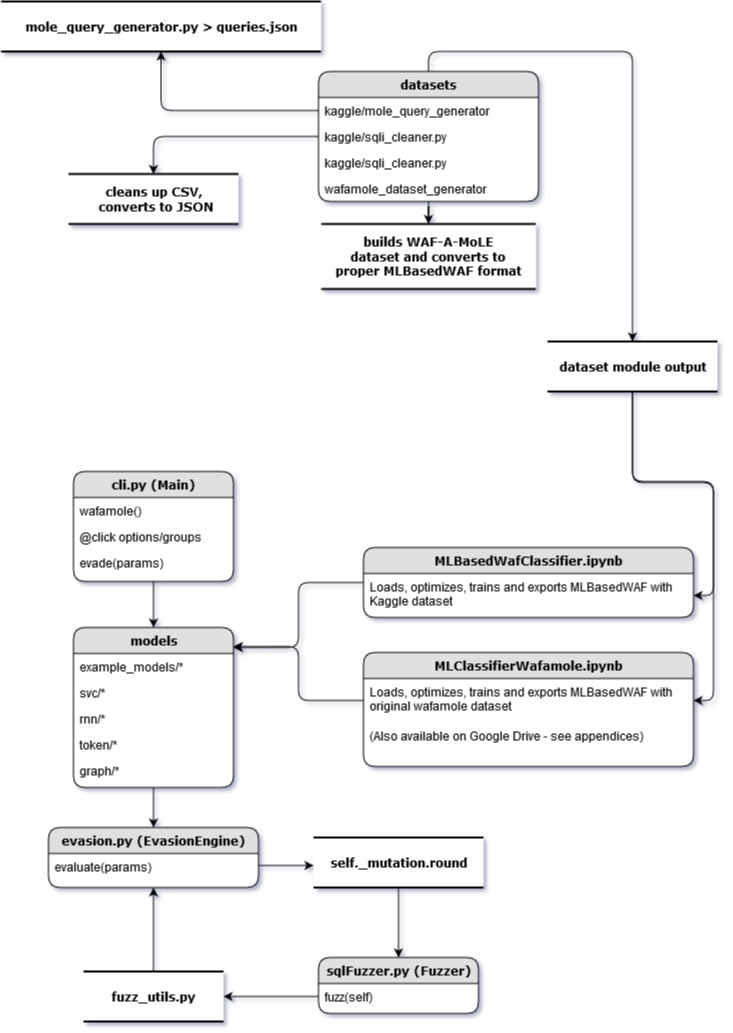
\includegraphics[width=16cm]{figuras/wafamole++_architecture.png} 
    \legend{Fonte: Elaboração Própria (2022)}
    \label{fig:internet} 
\end{figure}

\section{Operadores de Mutação}

O papel dos Operadores de Mutação tanto no WAF-A-MoLE quanto no wafamole++ é fundamental, atuando como as ferramentas para guiar as mudanças realizadas no \textit{payload} atual a cada iteração do algoritmo. Sendo assim, considerando-se como o primeiro desenvolvimento feito na extensão do programa original, o wafamole++ conta com três novos operadores de mutação adicionados ao montante original. Todos estes encontram-se agrupados na classe \verb+sqlfuzzer.py+, localizada na pasta \textbf{payloadfuzzer} da aplicação.

A presença destes incrementa a variedade de exemplos adversariais gerados, e em certos casos foi associado com uma rapidez maior na geração de queries finais. O primeiro destes é o \verb+shuffle_integers+, amostrado a seguir.

\label{sec:codigos}
\includecode[C]{Operador de mutação shuffle integers} {alg:codigo2}{codigos/operadores/shuffle_integers.py}

\bigskip

Sua implementação é a mais simples dentre os operadores novos - consistindo apenas na troca de números presentes no payload atual que lidera a fila principal por números inteiros diferentes entre 0 e 9. Selecionam-se números no payload (denominados de candidatos), a posição dos mesmos e seus conteúdos são armazenados e então uma substituição aleatória é escolhida e o payload modificado é retornado.  Interessantemente, modificando-se uma parte desse funcionamento para trocar a base numérica entre binário, octal, decimal e hexadecimal, obtém-se o próximo operador de mutação, com uma performance mais robusta. Trata-se do \verb+shuffle_bases+.

\label{sec:codigos}
\includecode[C]{Operador de mutação shuffle bases} {alg:codigo3}{codigos/operadores/shuffle_bases.py}

\bigskip

Nessa função a seleção e armazenamento de posições a serem modificadas é virtualmente idêntico - porém a substituição conta com uma lista de modificações em potencial dentre as quais uma é amostrada aleatoriamente na hora de ser realizada a mutação. Também são considerados os casos em que a mutação não ocasiona em variações no payload final. Finalmente, há o \verb+spaces_to_symbols+ - o operador com a performance mais interessante.

\label{sec:codigos}
\includecode[C]{Operador de mutação spaces to symbols} {alg:codigo3}{codigos/operadores/spaces_to_symbols.py}

\bigskip


\section{Modelos e WAFs avaliados}

\subsection{WAF-Brain}

\textbf{Autores}: Sergio D Fdez, cr0hn, Enrique Garcia. Disponível no Github \href{https://github.com/BBVA}{BBVA}

O WAF-Brain foi um dos primeiros firewalls a serem testados pela equipe do WAF-A-MoLE, e subsequentemente é o primeiro modelo de exemplo disponibilizado para testes na documentação do mesmo. Dessa maneira, foi extensivamente testado com os novos operadores de mutação, sendo de grande ajuda para diagnosticar os incluídos no wafamole++.

\begin{figure}[ht]
    \centering
    \caption{Dependências e logomarca do WAF-Brain}
    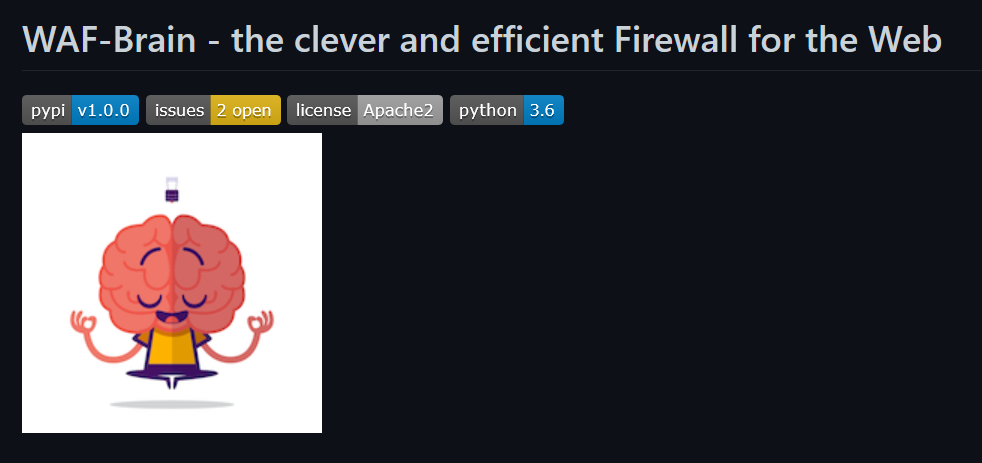
\includegraphics[width=12.5cm]{figuras/WAFBrain.png} 
    \legend{Fonte: \href{https://github.com/BBVA}{Github} (2019, p. TO-DO)}
    \label{fig:internet} 
\end{figure}

Seu funcionamento se dá, como anteriormente mencionado, através da estratégia de Deep Learning com Redes Neurais, pela qual são analisados cada campo de um determinado pedido HTTP sob a ótica de um classificador treinado desta maneira, determinando se esse campo é malicioso ou não.

Na adaptação WAF-A-MoLE, esse poder de predição é aproveitado exclusivamente na forma de probabilidade - tendo a probabilidade de ser uma SQL-Injection acima de um determinado limite, temos um caso malicioso. Isso requer que o classificador treinado no modelo não apenas mostre a previsão, mas também a precisa probabilidade com a qual chegou à mesma.

Por mais que se trate de um algoritmo sofisticado por natureza, surpreendentemente o WAF-Brain fora implementado pelos seus autores originais de uma maneira simplória o suficiente para ser um dos WAFs mais vulneráveis às estratégias de fuzzing do WAF-A-MoLE. Vários operadores de mutação isolados conseguem resultados frutíferos em pouco tempo, como será visto na seção de testes adiante.

\subsection{SQLiGoT}
Conforme uma advertência no repositório do WAF-A-MoLE pelos autores, esse Web Application Firewall exige um tempo de semanas para ser penetrado pela aplicação. Além disso, seu código encontra-se inacessível, proibindo a experimentação para o escopo desse trabalho, impossibilitando até mesmo que sejam feitas as etapas de treinamento. Por esse motivo, o SQLiGOT foi dispensado como alvo de estudo.

\subsection{MLBasedWAF}
Todos os modelos implementados tiveram como base o firewall ML-Based-WAF, disponível por vladan-stojnic no \href{https://github.com/vladan-stojnic/ML-based-WAF}{Github} que fora o WAF open source mais promissor e mais plausível de adaptar. Sua performance também era factível no contexto de recursos disponíveis para a conclusão deste projeto final.

\begin{figure}[ht]
    \centering
    \caption{Repositório ML-Based-WAF}
    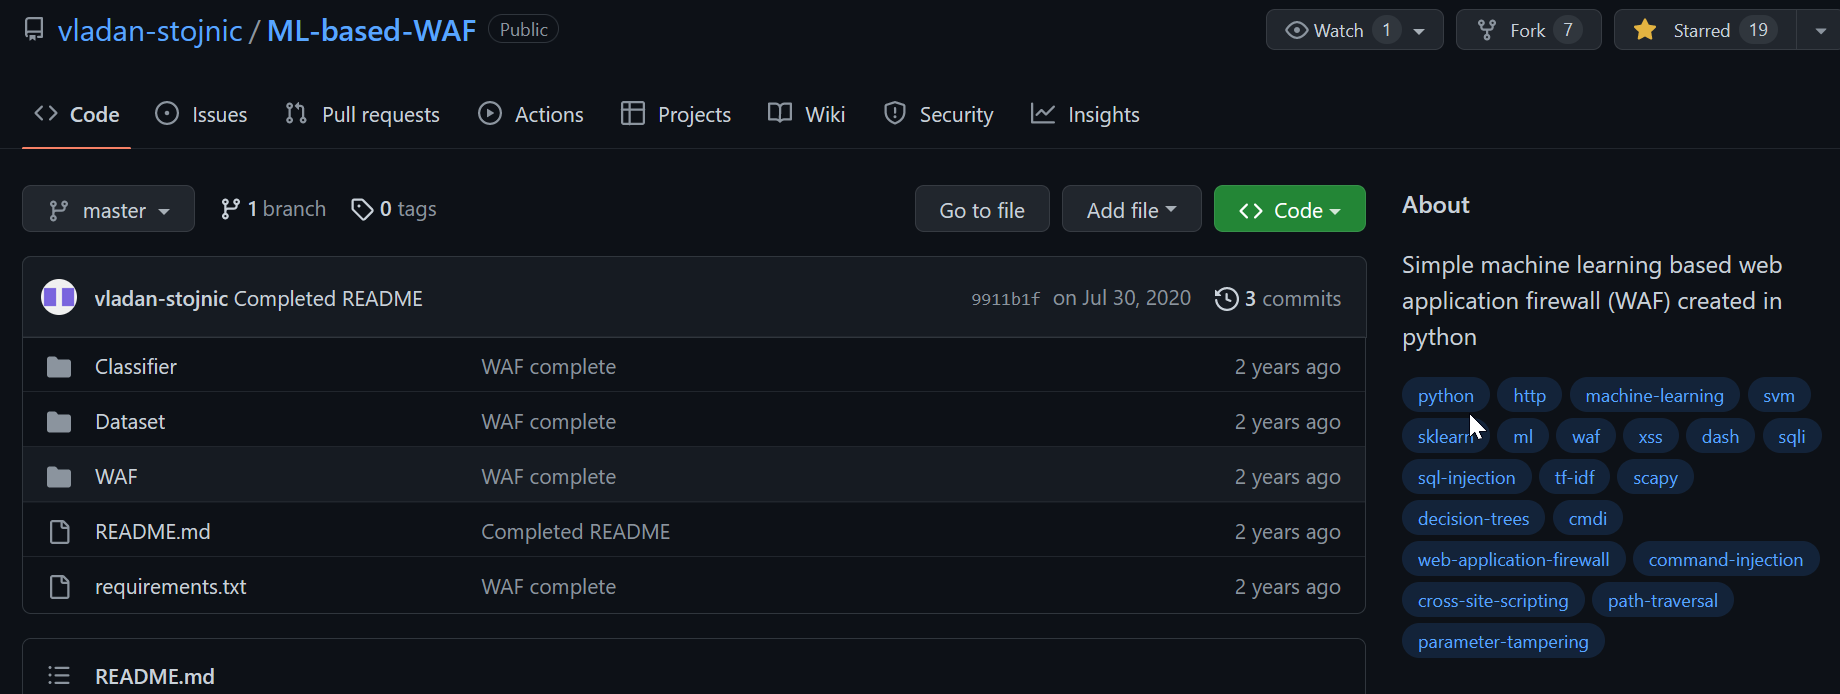
\includegraphics[width=16cm]{figuras/MLBasedWAF.png} 
    \legend{Fonte: \href{https://github.com/vladan-stojnic/ML-based-WAF}{Github} (2020, p. TO-DO)}
    \label{fig:internet} 
\end{figure}

Embora seja um WAF orientado ao tráfego real ou simulado de uma rede de fato, avaliando parâmetros HTTP em tempo real no seu componente sniffer.py tanto por SQL-Injections como por outras formas de ataque (XSS, cmdi e outras), ainda foi possível restringir seu funcionamento para adaptá-lo ao wafamole++. 

Para tal, foi necessário prever uma estratégia própria de treinamento para o classificador, além de um conjunto de dados especial para o mesmo. É cabível mencionar, no entanto, que isso introduziu uma série de dificuldades uma vez que sua documentação era consideravelmente modesta, e o banco novo a ser usado deveria seguir o padrão de formatação seguido pelo WAF.

Dentre as opções de datasets disponíveis com SQL Injections, foi escolhido inicialmente a versão SQLiV3.json da coleção do Kaggle, que fora anteriormente mencionada na seção de Arquitetura do wafamole++.

\begin{figure}[ht]
    \centering
    \caption{Detalhes Dataset SQL Injection Kaggle.}
    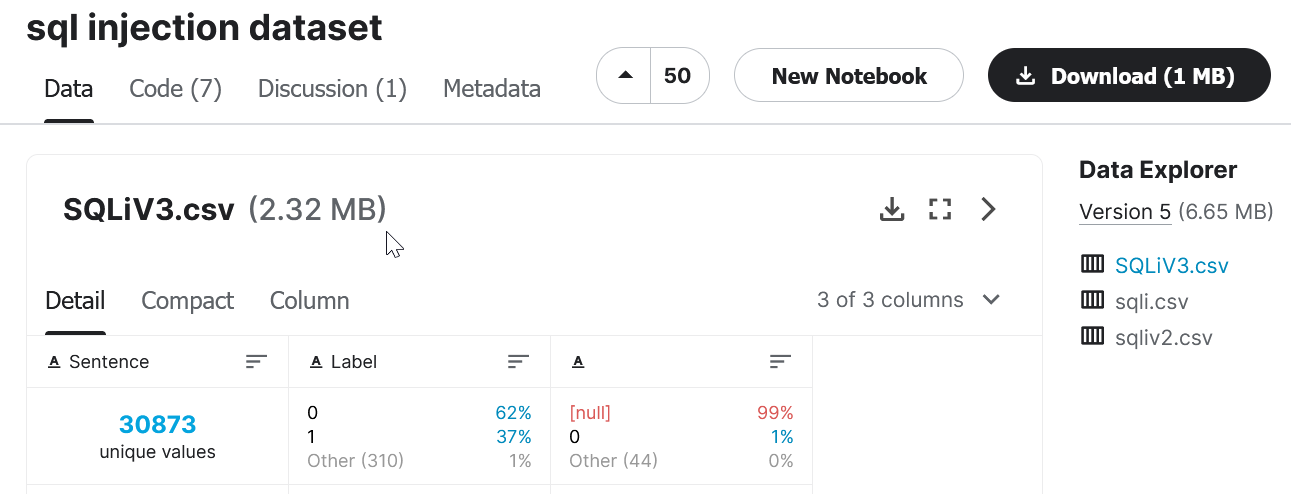
\includegraphics[width=16cm]{figuras/sqlInjectionDataset.png} 
    \legend{Fonte: \href{https://www.kaggle.com/datasets/syedsaqlainhussain/sql-injection-dataset}{Kaggle} (2021, p. TO-DO)}
    \label{fig:internet} 
\end{figure}

A etapa de correção de uma variedade de erros de formatação, polimento algumas queries incorretas (e de difícil proveito), e adaptação para o padrão .json utilizado pelo WAF, encontra-se codificada na função auxiliar \verb+sql_cleaner.py+.


\label{sec:codigos:sqli_cleaner}
\includecode[C]{Para tratamento de dados brutos} {alg:codigo3}{codigos/sqli_cleaner.py}
\bigskip


\subsection{Support Vector Machine}
Este foi o primeiro modelo implementado no wafamole++, antes do recebimento do dataset original da equipe original. Dado isso, esse classificador foi implementado com êxito usando os datasets \verb+SQLiV3.json+, \verb+SQLiV4.json+ e \verb+SQLiV5.json+. Tais datasets correspondem, respectivamente, aos seguintes modelos:
\begin{alineas}
\item \verb+test_svc_classifier_no_mole.dump+

(equivalente ao \verb+svc_trained.dump+);
\item \verb+test_svc_classifier_moled.dump+;
\item \verb+test_svc_classifier_extra_moled.dump+ 
\end{alineas}

A nomenclatura \textit{moled} foi escolhida para mensurar o quão reforçado o dataset usado no treinamento é - sendo tal reforço definido como a quantia de queries fuzzeadas pelo wafamole++ acrescentadas ao dataset inicial. E é evidente uma diferença na performance de cada modelo gerado - observou-se uma progressão de aumento (em média) de rodadas mutacionais (consumidas durante a execução) para os dois últimos modelos, especialmente no último.

Infelizmente um dos pontos de dificuldades foi o treinamento de um classificador deste tipo para o dataset original do WAF-A-MoLE, recebido após os testes iniciais. Em suma, tempos de execução excederam 48 horas em alguns casos, impossibilitando a conclusão da função \verb+fit+ de treinamento, mesmo com o backend de paralelização \verb+ray+.  Com isso foram feitas pesquisas subsequentes que revelaram uma possível inadequação desse classificador ao tipo de dado fornecido, sugerindo que outros classificadores sejam usados em seu lugar.

Além da testagem em cima do reforço via wafamole++, estruturalmente buscou-se diferenciar a implementação de Support Vector Machine da utilizada anteriormente no WAF-A-MoLE. Alguns parâmetros foram modificados, e fazendo-se uso de uma busca \textit{paramgrid} (para testar exaustivamente combinações de parâmetros) complementada de experimentação após sua execução, foi possível obter uma configuração com uma série de parâmetros diferentes.

Nesse contexto destaca-se um que troca o algoritmo fundamental por trás do Support Vector Machine por um com abordagem não linear (no caso, \verb+kernel = 'rbf'+) em contraste direto com o algoritmo linear empregado no modelo Token-based padrão do WAF-A-MoLE. Por fim, é amostrado sua célula de código principal contida no Python Notebook.

\label{sec:codigos:modelos}
\includecode[C]{Pipeline classificador SVC Não-Linear}{alg:codigo3}{codigos/modelos/svc_model_sqliv3.py}
\bigskip

\subsection{Stochastic Gradient Descent}
O segundo modelo a ser codificado pôde ser testado tanto para os datasets do kaggle como do WAF-A-MoLE original, sem grandes problemas de performance. No caso posterior, de fato houve uma exigência maior da máquina, requerindo um ambiente com mais memória que o desktop originalmente usado para executar os notebooks. Com isso, foi empregada a plataforma Google Colaboratory, da subdivisão de pesquisa da Google. 

Essa mudança de ambiente ocasionou em uma série de vantagens, dentre as quais destacam-se: uma maior facilidade em executar um ambiente minimamente funcional, disponibilização de um link facilmente compartilhável, colaboração simultânea e principalmente mais memória RAM para executar as pipelines de treinamento. 

Um fator indesejável é a impossibilidade de gerenciar com maior precisão a versão de Python e algumas dependências - ocasionando numa séria poluição de logs em virtude da deprecação de algumas técnicas empregadas em versões antigas dos pacotes \verb+numpy+, \verb+scikit-learn+ e \verb+tensorflow+, dificultando o desenvolvimento e diagnóstico de erros. 

Acredita-se que a principal falha da plataforma, no entanto, seja a limitação de sua versão gratuita, no entanto, que desliga todas as células do Notebook em uso após um período fixo de 12 horas, a menos que o usuário esteja ativamente codificando na mesma. Isso dificultou grandemente o modelo discutido anteriormente, cujo fluxo de execução excedia facilmente esse intervalo para datasets suficientemente grandes.

Não obstante, no caso do Stochastic Gradient Descent a performance foi satisfatória o suficiente para gerar um par de modelos a serem testados: um para o dataset \verb+SQLiV5.json+, entitulado de \verb+sgd_trained.dump+ e um para o dataset WAF-A-MoLE, \verb+test_sgd_classifier.py+. A performance dos mesmos será comparada mais detalhadamente no capítulo de testes adiante. 

\label{sec:codigos:modelos}
\includecode[C]{Pipeline classificador SGD sem backend de paralelização ray (Para SQLiV5.json)}{alg:codigo3}{codigos/modelos/sgd_model_sqliv3.py}
\bigskip

\subsection{Ada Boost Classifier}

O último modelo, e um dos mais interessantes, é o Ada Boost Classifier, implementado apenas para o dataset do WAF-A-MoLE no final da implementação do trabalho. Sua performance é consideravelmente promissora, superando alguns dos modelos padrões do WAF-A-MoLE como alguns dos baseados em Token e o WAF-Brain. Para treiná-lo, foi necessário o uso do backend de paralelização \verb+ray+, tomando ainda um tempo considerável de vários minutos.

O resultado desse modelo é entitulado de \verb+test_ada_classifier.dump+. Abaixo é amostrado como é feita essa adaptação.

\label{sec:codigos:modelos}
\includecode[C]{Pipeline classificador Ada Boost com backend de paralelização ray}{alg:codigo3}{codigos/modelos/ada_model.py}
\bigskip

Por fim, para cada um desses novos modelos funcione, é necessária a criação de uma classe \textit{Wrapper} para servir de ponte entre a pipeline gerada pela biblioteca \verb+joblib+ e o wafamole++. A mesma inclui dois métodos: \verb+extract_features()+, atuando como uma função identidade; e \verb+classify()+, que realiza a classificação de fato sempre através da função \verb+predict_proba()+ que é requerida nos parâmetros de todos os modelos. Essa função retorna, conforme o comentário no código abaixo, a probabilidade do payload \verb+value+ de ser uma injeção SQL. Essa probabilidade é a que é comparada com a \verb+threshold+ limite dada pelo usuário no início da execução do programa, para uma eventual condição de parada.

\label{sec:codigos:modelos}
\includecode[C]{Classe SVCClassifierWrapper para modelos novos}{alg:codigo3}{codigos/modelos/svc_wrapper.py}
\bigskip



